\documentclass{libs/XJTLU_format}
% Inserting the preamble file with the packages
%%%%%%%%%%%%%%%%%%%%%%%%%%%%%%%%%%%%%%%%%%%%%%%%%%%%%%%%%%%%%%%%%%%%%
%% This file contains the packages that can be used in the beamer. %%
%%%%%%%%%%%%%%%%%%%%%%%%%%%%%%%%%%%%%%%%%%%%%%%%%%%%%%%%%%%%%%%%%%%%%
% Package to fonts family
\usepackage[T1]{fontenc}
% Package to accentuation
\usepackage[utf8]{inputenc}
% Package to Figures
\usepackage{graphicx}
% Package to the colors
\usepackage{color}
% Package to the colors
\usepackage{xcolor}
% Packages to math symbols and expressions
\usepackage{amsfonts, amssymb, amsmath}
% Package to multiple lines and columns in table
\usepackage{multirow, array} 
% Package to create pseudo-code
% For more detail of this package: http://linorg.usp.br/CTAN/macros/latex/contrib/algorithm2e/doc/algorithm2e.pdf
\usepackage{algorithm2e}
% Package to insert code
\usepackage{listings} 
\usepackage{keyval}
% Package to justify text
\usepackage[document]{ragged2e}
% Package to manage the bibliography
\usepackage[backend=biber, style=numeric, sorting=none]{biblatex}
% Package to facilities quotations
\usepackage{csquotes}
% Package to use multicols
\usepackage{multicol}
\usepackage{transparent}

% Inserting the references file

\usepackage [spanish]{babel}
\usepackage [utf 8]{inputenc}

% Title
\title[Curso Análisis exploratorio de datos en Python y R]{\huge\textbf{Curso Análisis exploratorio de datos en Python y R}}
% Subtitle
\subtitle{Descarga e instalación}
% Author of the presentation
\author{Juan Camilo Perdomo}
% Institute's Name
\institute[Universidad del Rosario]{
    % email for contact
    \normalsize{\email{juan.perdomor@urosario.edu.co}}
    \newline
    % University name
    \university{Universidad del Rosario}
    \newline
    % Department Name
    \department{Bogotá, Colombia}
}
% date of the presentation
\date{\today}

%%%%%%%%%%%%%%%%%%%%%%%%%%%%%%%%%%%%%%%%%%%%%%%%%%%%%%%%%%%%%%%%%%%%%%%%%%%%%%%%%%
\begin{document}
% insert the code style
%%%%%%%%%%%%%%%%%%%%%%%%%%%%%%%%%%%%%%%%%%%%%%%%%%%%%%%%%%%%%%%%%%%%%%%%%%%%%%%%%%%
%% This file contains the style of the codes show in slides.                     %%
%% The package used is listings, but it possible to used others.                 %%
%%%%%%%%%%%%%%%%%%%%%%%%%%%%%%%%%%%%%%%%%%%%%%%%%%%%%%%%%%%%%%%%%%%%%%%%%%%%%%%%%%%

% color used in the code style
\definecolor{codegreen}{rgb}{0,0.6,0}
\definecolor{codegray}{rgb}{0.5,0.5,0.5}
\definecolor{codepurple}{rgb}{0.58,0,0.82}
\definecolor{codebackground}{rgb}{0.95,0.95,0.92}

% style of the code!
\lstdefinestyle{codestyle}{
    backgroundcolor=\color{codebackground},   
    commentstyle=\color{codegreen},
    keywordstyle=\color{magenta},
    numberstyle=\tiny\color{codegray},
    stringstyle=\color{codepurple},
    basicstyle=\ttfamily\footnotesize,
    frame=single,
    breakatwhitespace=false,         
    breaklines=true,                 
    captionpos=b,                    
    keepspaces=true,                 
    numbers=left,                    
    numbersep=5pt,                  
    showspaces=false,                
    showstringspaces=false,
    showtabs=false,                  
    tabsize=2,
    title=\lstname 
}

\lstset{style=codestyle}



%% ---------------------------------------------------------------------------
% First frame (with tile, subtitle, ...)
\begin{frame}{}
    \maketitle
\end{frame}

%% ---------------------------------------------------------------------------
% Second frame
\begin{frame}{Tabla de contenidos}
    \tableofcontents
\end{frame}

%% ---------------------------------------------------------------------------
\section{Introducción}

\begin{frame}[fragile] 
    \frametitle{Introducción}
    \begin{center}
        En esta sección descargaremos los programas y/o aplicaciones básicos y más comúnes para trabajar con los lenguajes de R y Python. Como se mencionó en la anterior clase estos son: R-Studio, en el caso de R, y el Jupyter Notebook (por ahora, el incluido en el paquete de Anaconda), en el caso de Python. Sin embargo, para hacer uso de estos Entornos de Desarrollo Integrado (IDE, por sus siglas en inglés), es necesario, o al menos deseable, instalar previamente los programas o software que contienen los lenguajes o códigos de Python y R propiamente dichos. \newline
    \end{center}
\begin{multicols}{4}
        \begin{figure}[H]
            
\includegraphics [width =0.15\textwidth]{r.png}
        \end{figure}
        \begin{figure}[H]
            
\includegraphics [width =0.25\textwidth]{RStuido.png}
        \end{figure}
        \begin{figure}[H]
            
\includegraphics [width =0.2\textwidth]{python.png}
        \end{figure}
        \begin{figure}[H]
            
\includegraphics [width =0.1\textwidth]{Jupyter.png}
        \end{figure}
\end{multicols}

\end{frame}

%% ---------------------------------------------------------------------------
\section{Instalación de R y R studio}

\begin{frame}[fragile] 
    \frametitle{Instalación de R} 
    Para la instalación de R, es necesario ingresar al siguiente link: {\color{blue}\url{https://cran.r-project.org/}}
        \begin{figure}[H]
            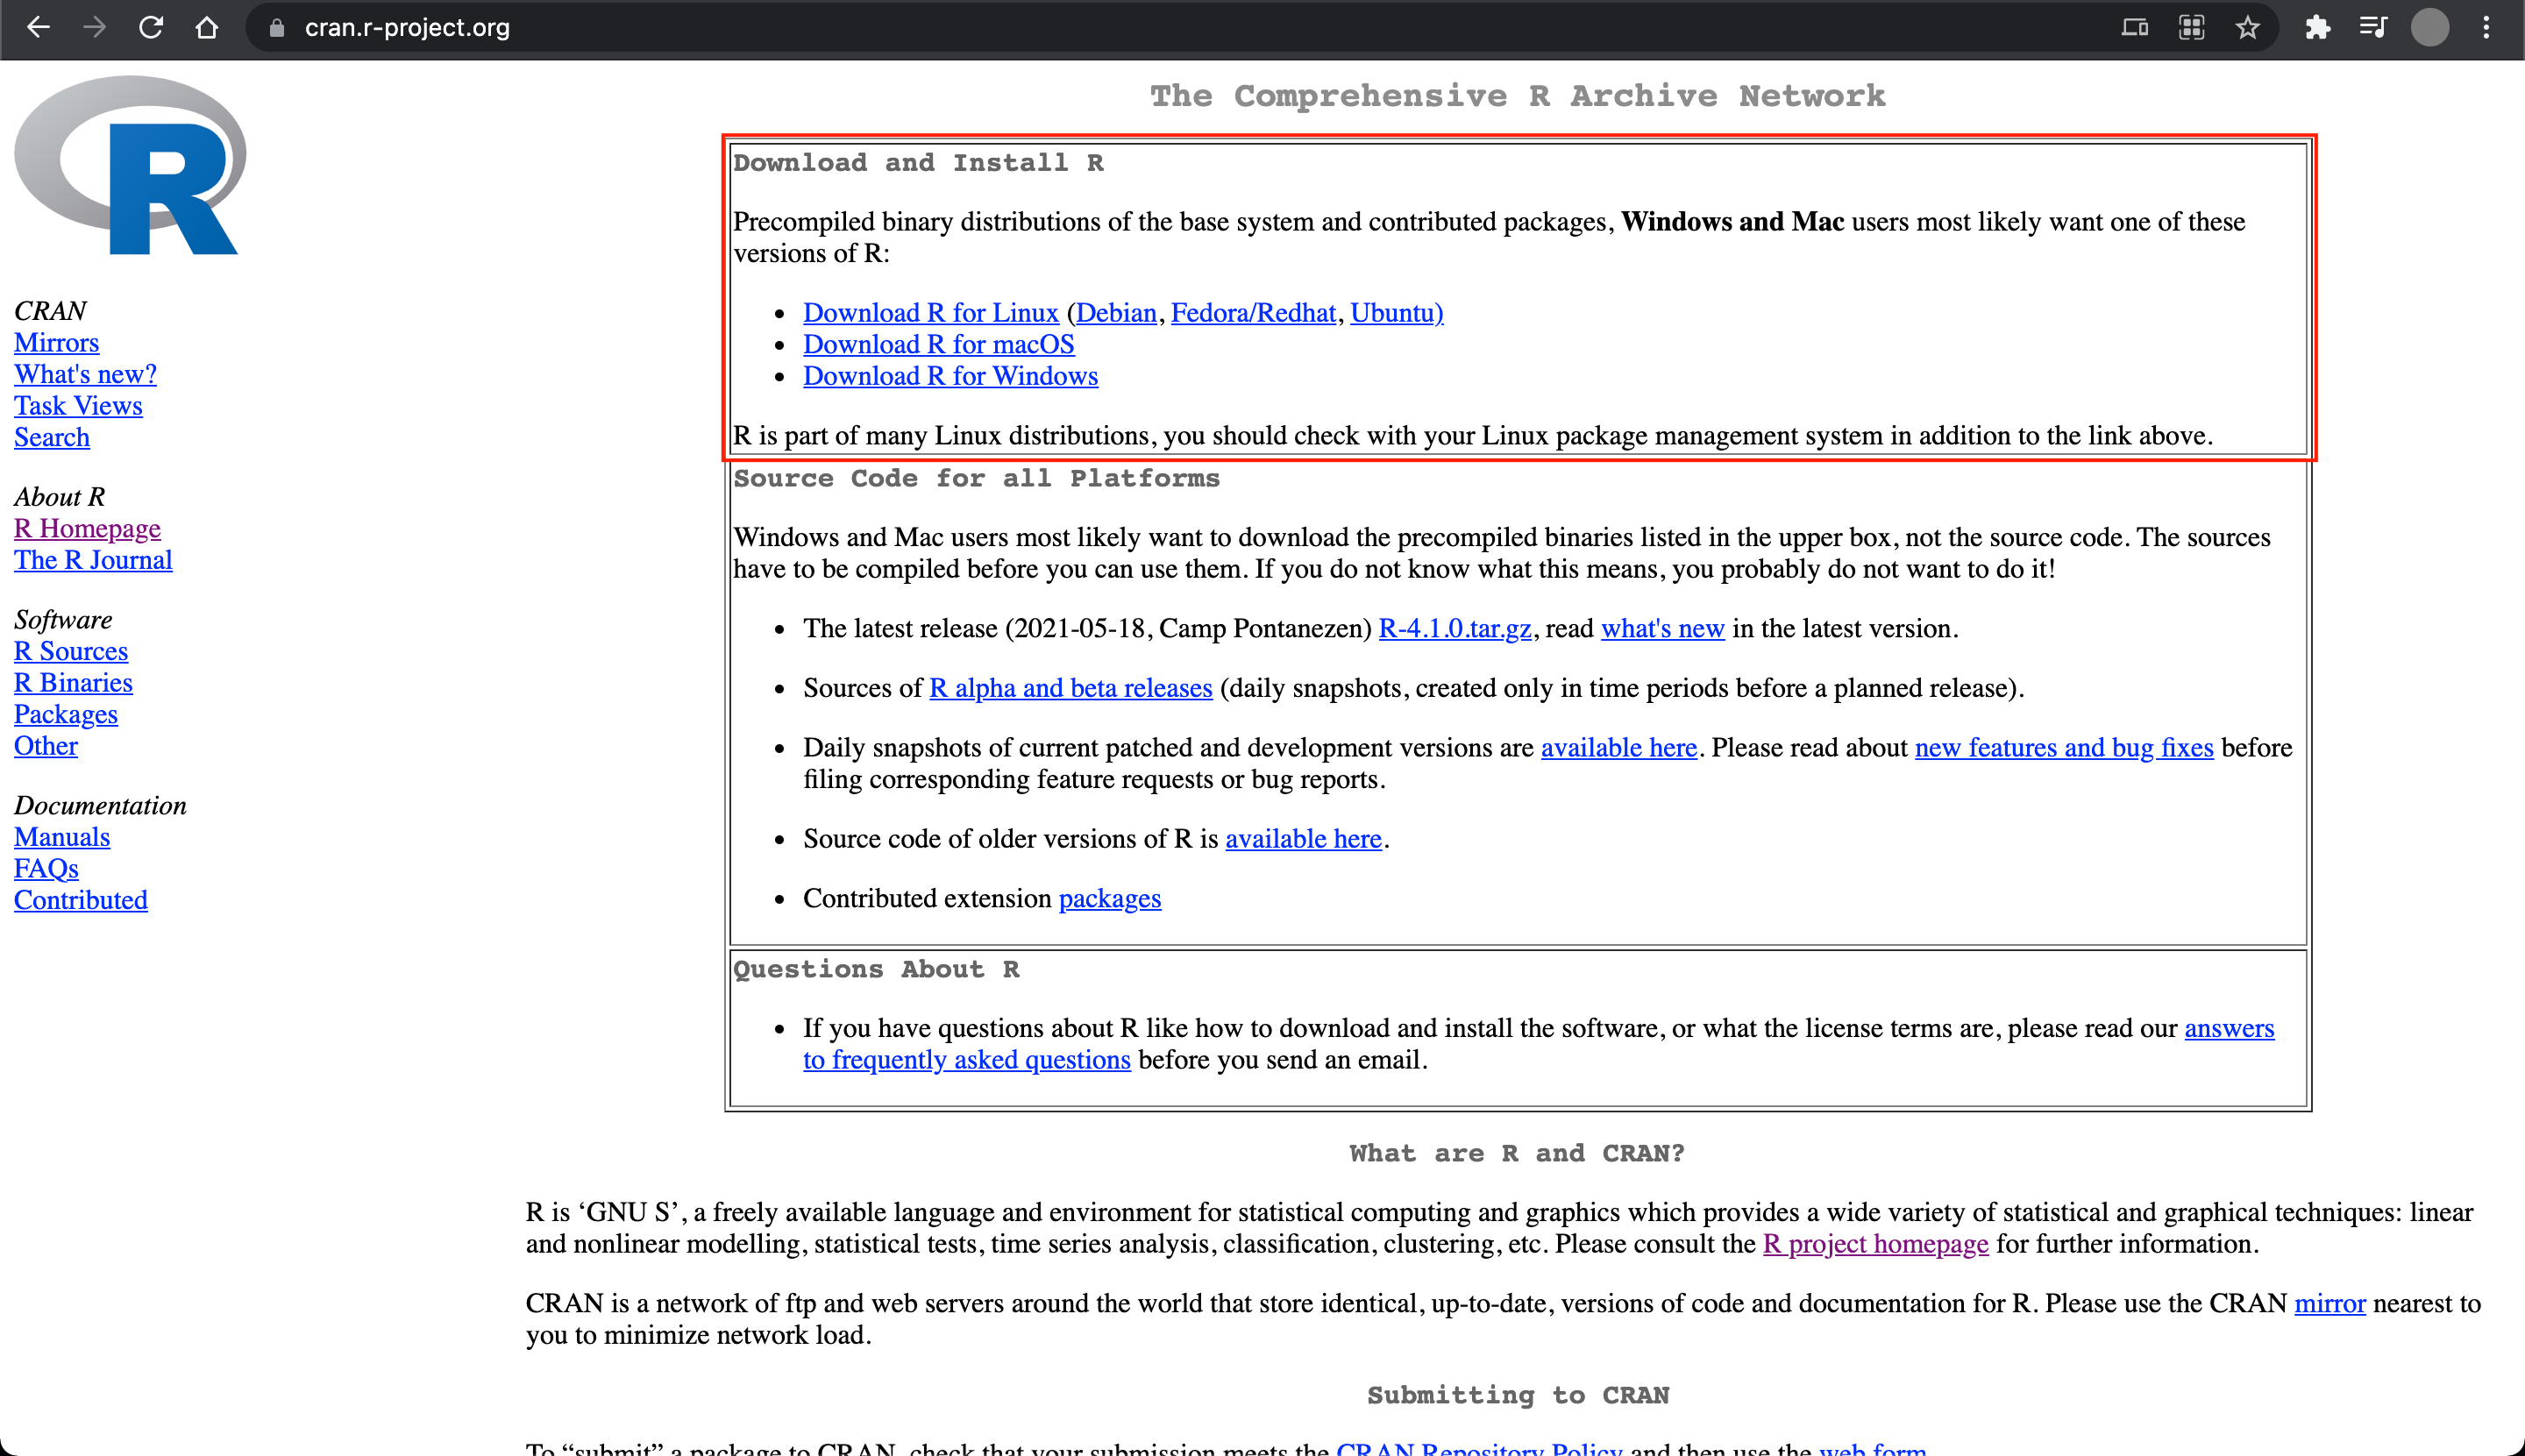
\includegraphics [width =0.7\textwidth]{InstalaR.png}
        \end{figure}
    Se descarga el instalador, según el sistema operativo que se maneje y se siguen los pasos básicos de intalación.
\end{frame}
%% ---------------------------------------------------------------------------
\begin{frame}[fragile] 
    \frametitle{Instalación de R studio} 
    Para la instalación de R-Studio, es necesario ingresar al siguiente link: {\color{blue}\url{https://www.rstudio.com/products/rstudio/download/}}
        \begin{figure}[H]
            \includegraphics [width =0.7\textwidth]{InstalaRstudio.png}
        \end{figure}
    Se descarga el instalador, según el sistema operativo que se maneje y se siguen los pasos básicos de intalación.
\end{frame}
%% ---------------------------------------------------------------------------
\section{Instalación de Python y Anaconda}
\begin{frame}[fragile] 
    \frametitle{Instalación de Python} 
    Para la instalación de Python, es necesario ingresar al siguiente link: {\color{blue}\url{https://www.python.org/downloads/}}
        \begin{figure}[H]
            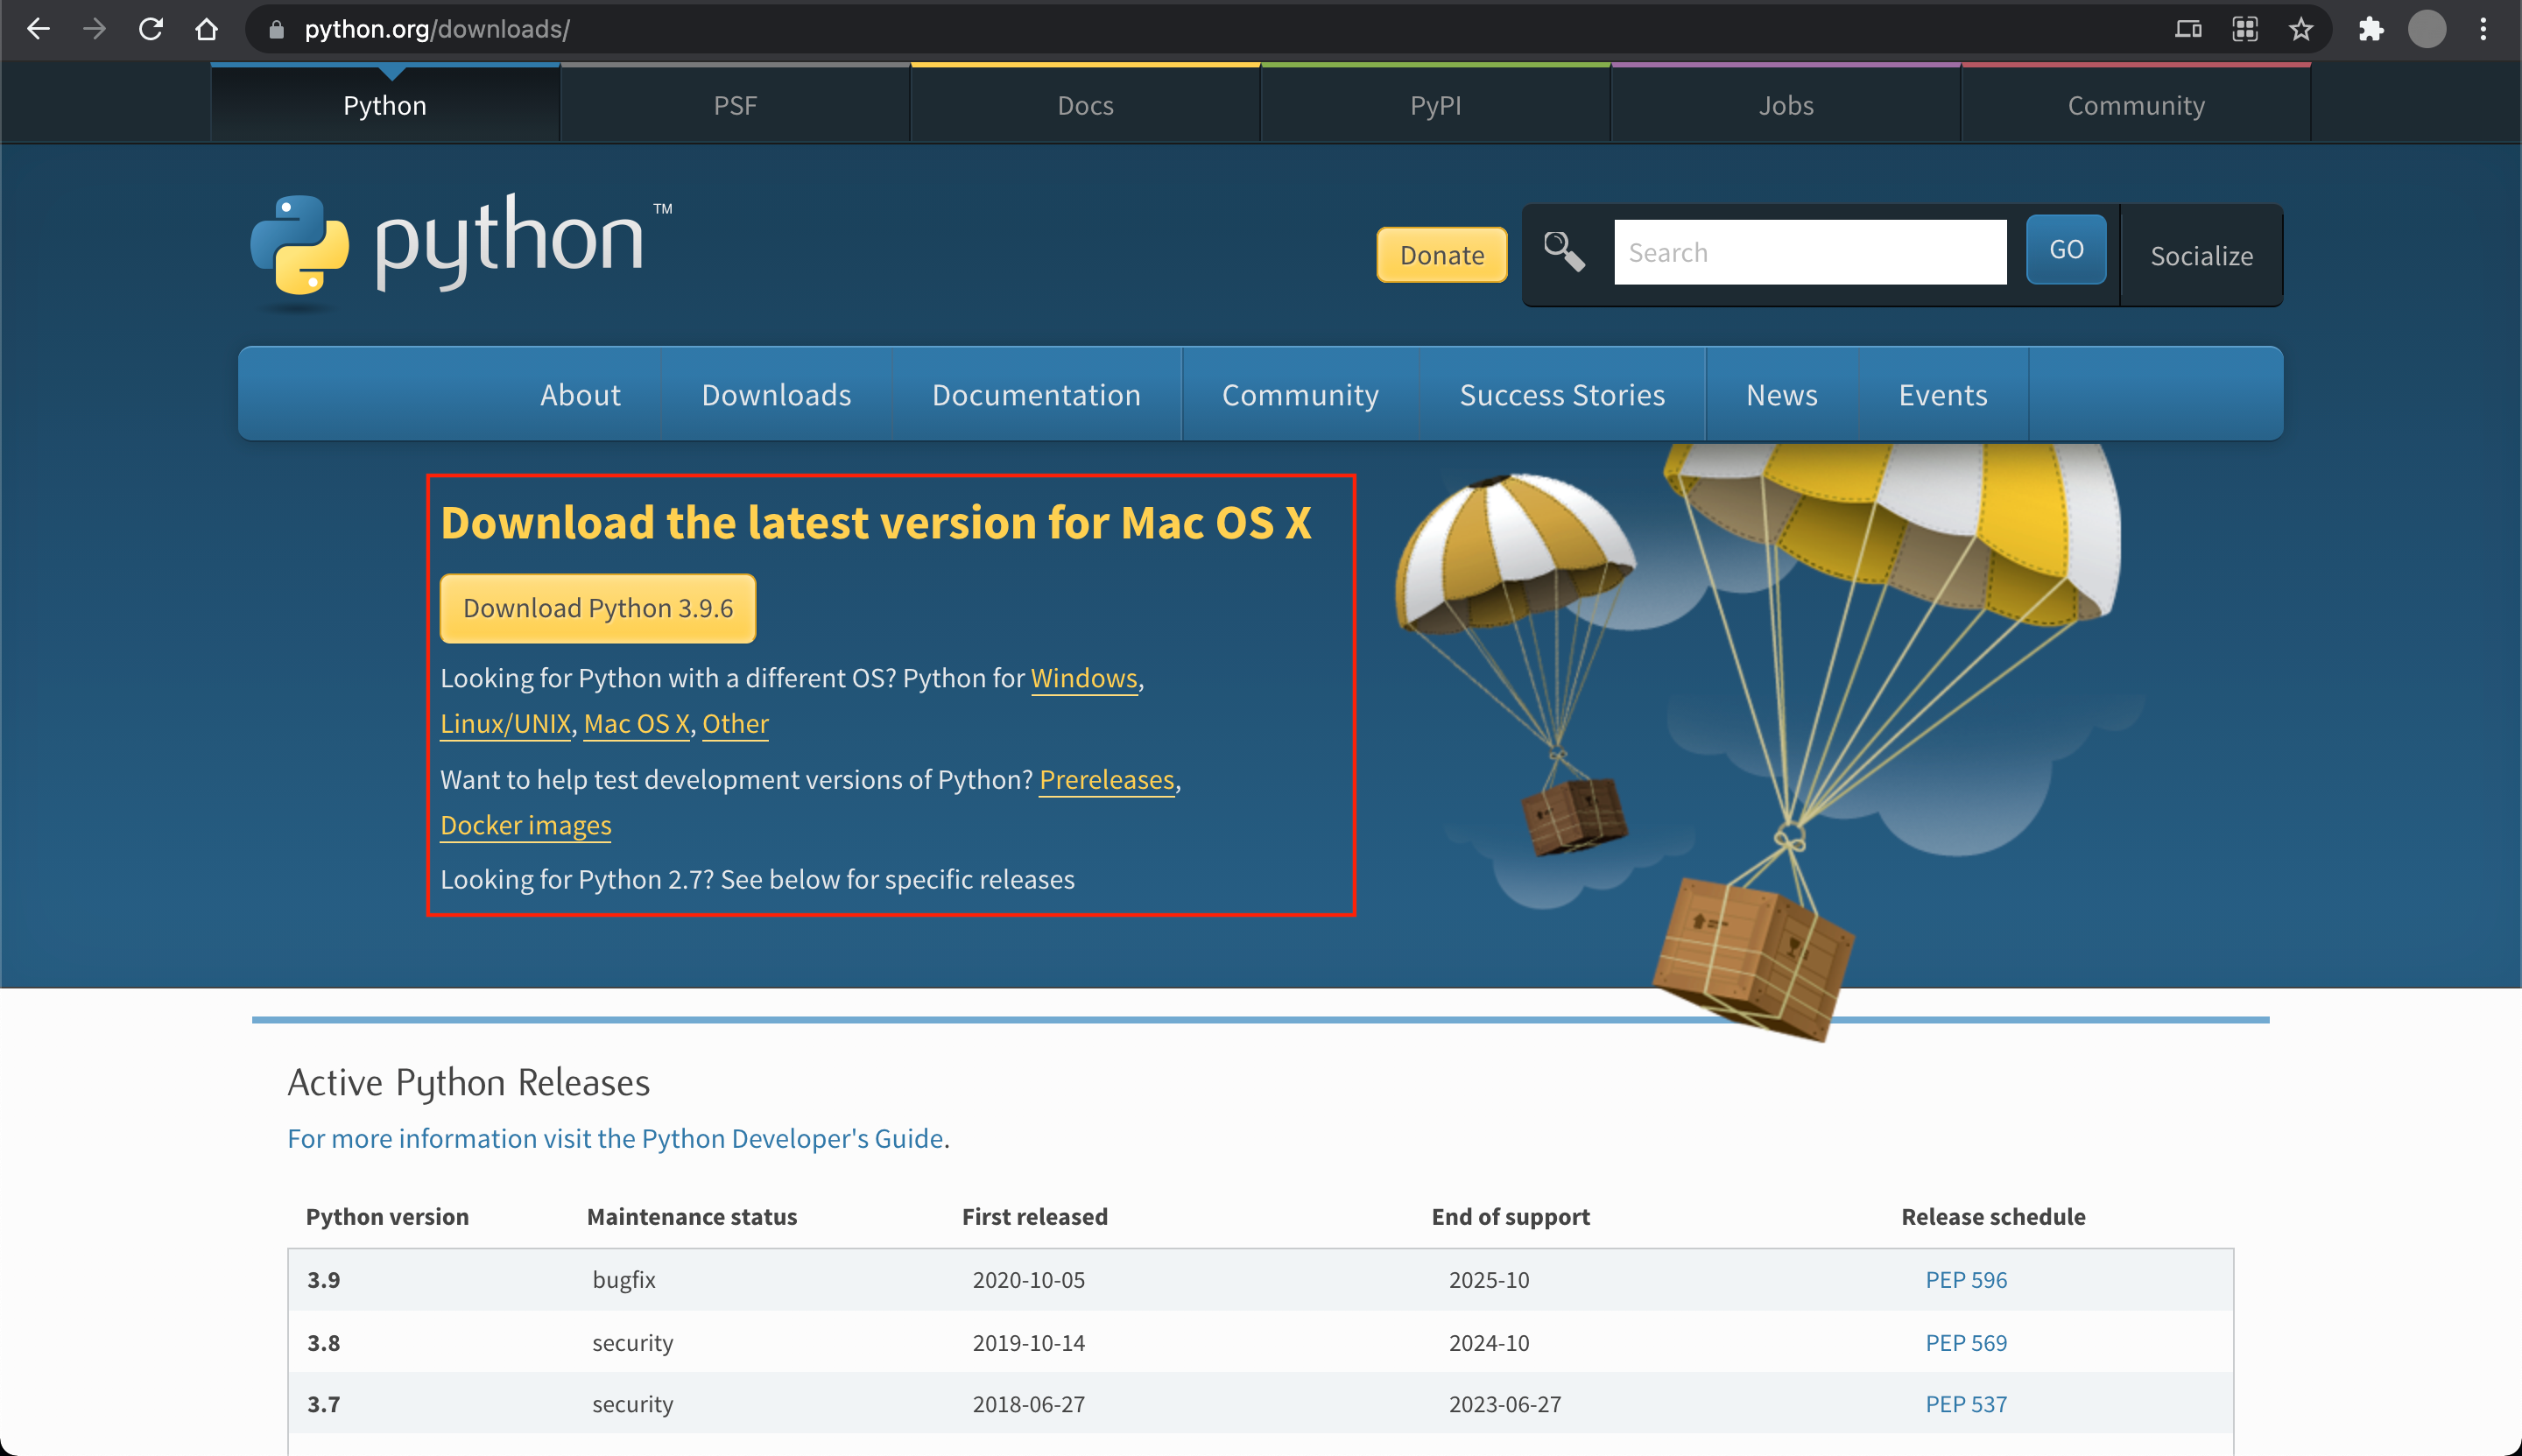
\includegraphics [width =0.7\textwidth]{InstaPy.png}
        \end{figure}
    Se descarga el instalador, según el sistema operativo que se maneje y se siguen los pasos básicos de intalación.
\end{frame}
%% ---------------------------------------------------------------------------

\begin{frame}[fragile] 
    \frametitle{Instalación de Anaconda} 
    Para la instalación de Anaconda, es necesario ingresar al siguiente link: {\color{blue}\url{https://www.anaconda.com//}}
        \begin{figure}[H]
            
\includegraphics [width =0.7\textwidth]{InstaAna.png}
        \end{figure}
    Dar click en la pestaña de -Products- y en -Individual edition-.
\end{frame}
%% ---------------------------------------------------------------------------

\begin{frame}[fragile] 
    \frametitle{Instalación de Anaconda} 
    Estos pasos llevan al siguiente link: {\color{blue}\url{https://www.anaconda.com/products/individual}}
        \begin{figure}[H]
            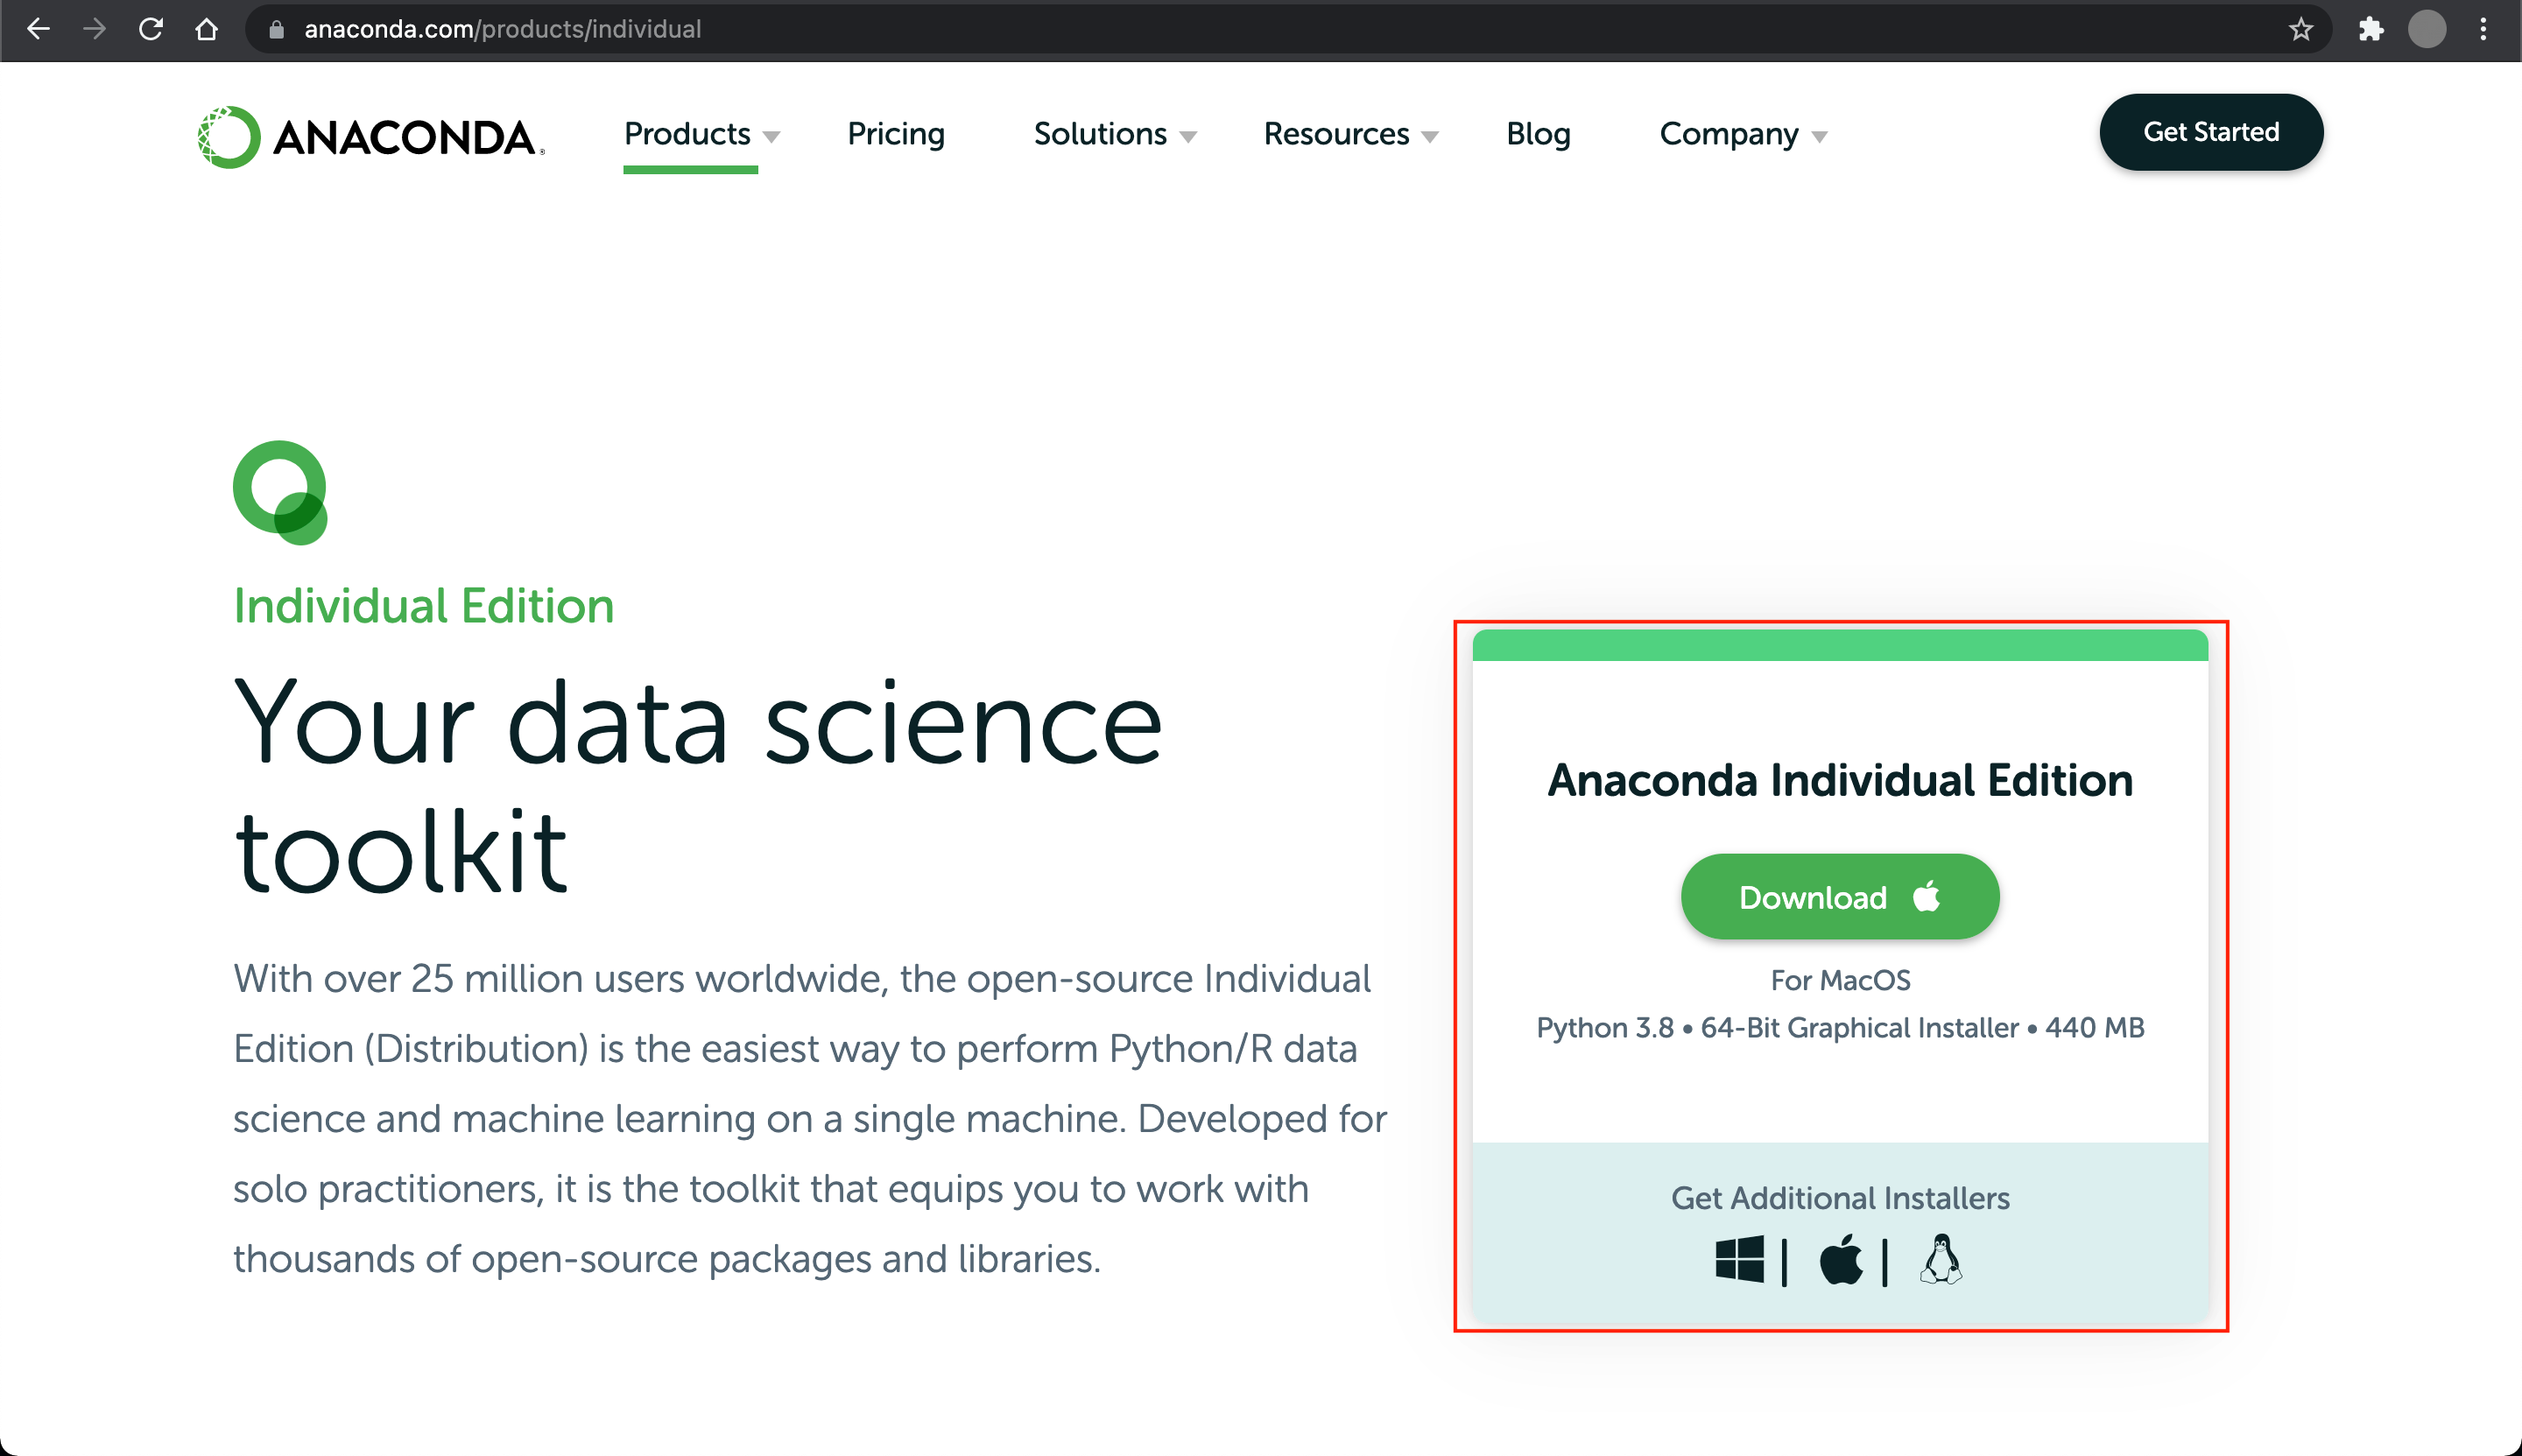
\includegraphics [width =0.7\textwidth]{Descarga.png}
        \end{figure}
    Se descarga el instalador, según el sistema operativo que se maneje y se siguen los pasos básicos de intalación.
\end{frame}
%% ---------------------------------------------------------------------------

\begin{frame}[fragile] 
    \frametitle{Instalación de Anaconda} 
    Aunque con este programa es importante tener en cuenta los siguientes pasos, según se use Windows o Mac.
    \begin{multicols}{2}
        \begin{figure}[H]
            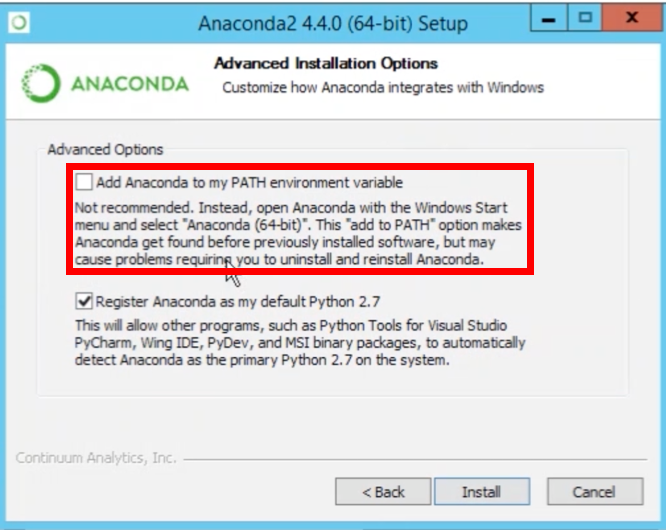
\includegraphics [width =0.484\textwidth]{Windows.png}
        \end{figure}
                \begin{figure}[H]
            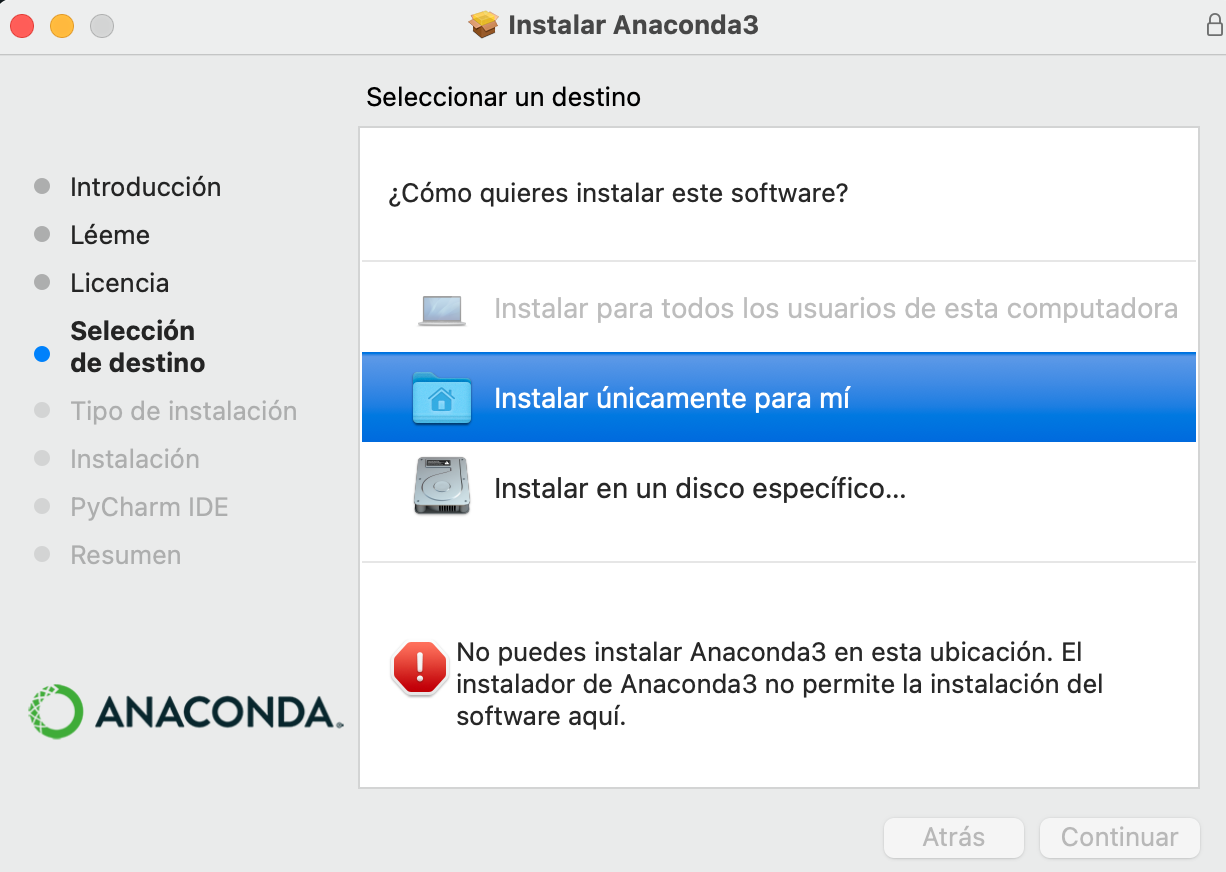
\includegraphics [width =0.528\textwidth]{Mac.png}
        \end{figure}
    \end{multicols}
    O hacer click en el siguiente link para acceder a más información: {\color{blue}\url{https://docs.anaconda.com/anaconda/install/}}
\end{frame}
%% ---------------------------------------------------------------------------
\end{document}